\documentclass[11pt]{article}
\usepackage[paperwidth=29.7cm,paperheight=16.7cm,left=12mm,right=12mm,top=10mm,bottom=12mm]{geometry}

% -----------------------------------------------------------------------------
% Fonts & Localization (XeLaTeX)
% -----------------------------------------------------------------------------
\usepackage{fontspec}
\usepackage{xunicode}
\usepackage{xltxtra}
\defaultfontfeatures{Mapping=tex-text}

\setmainfont{Bai Jamjuree}[
  UprightFont=* Regular,
  BoldFont=* SemiBold,
  ItalicFont=* Italic,
  BoldItalicFont=* SemiBold Italic
]

% -----------------------------------------------------------------------------
% Essential Packages
% -----------------------------------------------------------------------------
\usepackage{amsmath,amssymb,amsfonts}
\usepackage{booktabs}
\usepackage{tabularx}
\usepackage{colortbl}
\usepackage{xcolor}
\usepackage{graphicx}
\usepackage{enumitem}
\usepackage{fancyhdr}
\usepackage{hyperref}
\usepackage{caption}
\usepackage{tcolorbox}
\tcbuselibrary{skins,breakable}

% -----------------------------------------------------------------------------
% Color Palette: Modern DeepTech Startup (Navy, Electric Blue, Amber, Slate)
% -----------------------------------------------------------------------------
\definecolor{primary}{RGB}{15, 34, 64}        % Deep Midnight Navy
\definecolor{secondary}{RGB}{14, 116, 144}    % Deep Cyan
\definecolor{accent}{RGB}{217, 119, 6}        % Vibrant Amber / Gold
\definecolor{highlight}{RGB}{16, 185, 129}    % Emerald Green
\definecolor{lightbg}{RGB}{248, 250, 252}     % Slate 50
\definecolor{cardbg}{RGB}{255, 255, 255}
\definecolor{cardborder}{RGB}{226, 232, 240}
\definecolor{darkgray}{RGB}{30, 41, 59}       % Slate 800
\definecolor{danger}{RGB}{225, 29, 72}        % Crimson Red

\hypersetup{
  colorlinks=true,
  linkcolor=secondary,
  urlcolor=secondary
}

% -----------------------------------------------------------------------------
% Header & Footer Settings for 16:9 Slide Deck
% -----------------------------------------------------------------------------
\setlength{\headheight}{16pt}
\setlength{\headsep}{8pt}
\pagestyle{fancy}
\fancyhf{}
\renewcommand{\headrulewidth}{0.8pt}
\renewcommand{\footrulewidth}{0.5pt}
\fancyhead[L]{\small \textbf{\textcolor{primary}{NEXVIA AEGIS}} \textbar\ \textcolor{darkgray}{TED Fund Startup Pitch Deck}}
\fancyhead[R]{\small \textbf{\textcolor{accent}{โครงการยุววิสาหกิจเริ่มต้น (Youth Startup: โปรแกรม IDEA 150,000 บาท)}}}
\fancyfoot[L]{\footnotesize \textcolor{darkgray}{กองทุนพัฒนาผู้ประกอบการเทคโนโลยีและนวัตกรรม (กระทรวง อว.) \textbar\ ผู้เสนอ: ทีมวิจัย NEXVIA AEGIS}}
\fancyfoot[R]{\footnotesize \textbf{สไลด์ที่ \thepage\ / 10}}

\begin{document}

% =============================================================================
% SLIDE 1: Title & Executive Summary
% =============================================================================
\begin{tcolorbox}[colback=primary,colframe=primary,arc=4mm,boxrule=0pt,top=10mm,bottom=10mm,left=10mm,right=10mm]
  \begin{center}
    {\fontsize{24pt}{28pt}\selectfont \textbf{\textcolor{white}{NEXVIA AEGIS: The World's First Provably Safe Autonomy Engine}}}\\[4mm]
    {\fontsize{13pt}{16pt}\selectfont \textcolor{accent}{\textbf{ระบบเกราะความปลอดภัยปัญญาประดิษฐ์ที่รับประกันความปลอดภัย 100\% ทางคณิตศาสตร์ สำหรับอากาศยานและยานพาหนะอัตโนมัติ}}}\\[3mm]
    {\normalsize \textcolor{white}{ข้อเสนอโครงการขอรับทุน TED Fund โปรแกรมสร้างผู้ประกอบการใหม่ (IDEA: 150,000 บาท) — กระทรวง อว.}}
  \end{center}
\end{tcolorbox}

\vspace{2mm}
\begin{center}
\begin{tabularx}{\textwidth}{XXXX}
  \begin{tcolorbox}[colback=lightbg,colframe=cardborder,arc=2mm,top=3mm,bottom=3mm]
    \centering
    \textbf{\textcolor{primary}{ความพร้อมเทคโนโลยี}}\\[1mm]
    {\Large \textbf{\textcolor{highlight}{TRL 4 $\to$ TRL 6}}}\\[1mm]
    \footnotesize เริ่มต้นจาก Lab สู่สนาม EECi
  \end{tcolorbox} &
  \begin{tcolorbox}[colback=lightbg,colframe=cardborder,arc=2mm,top=3mm,bottom=3mm]
    \centering
    \textbf{\textcolor{primary}{การรับรองความปลอดภัย}}\\[1mm]
    {\Large \textbf{\textcolor{highlight}{ชน 0\% \textbar\ 0 Crashes}}}\\[1mm]
    \footnotesize ทดสอบ 2,880 โลกจำลอง
  \end{tcolorbox} &
  \begin{tcolorbox}[colback=lightbg,colframe=cardborder,arc=2mm,top=3mm,bottom=3mm]
    \centering
    \textbf{\textcolor{primary}{ความเร็ว C++ ไมโครเคอร์เนล}}\\[1mm]
    {\Large \textbf{\textcolor{highlight}{$<$ 0.04 ms}}}\\[1mm]
    \footnotesize Standalone C++20 Header-Only
  \end{tcolorbox} &
  \begin{tcolorbox}[colback=lightbg,colframe=cardborder,arc=2mm,top=3mm,bottom=3mm]
    \centering
    \textbf{\textcolor{primary}{ชุดทดสอบอัตโนมัติ}}\\[1mm]
    {\Large \textbf{\textcolor{highlight}{884 / 884 Tests}}}\\[1mm]
    \footnotesize ผ่านการทดสอบสมบูรณ์ 100\%
  \end{tcolorbox}
\end{tabularx}
\end{center}

\vspace{1mm}
\noindent \textbf{\textcolor{primary}{สรุปภาพรวมวิสัยทัศน์:}} NEXVIA AEGIS คือเทคโนโลยี DeepTech สัญชาติไทยที่คิดค้นขึ้นเพื่อแก้ปัญหาคอขวดของอุตสาหกรรมหุ่นยนต์:\\[1mm]
เปลี่ยนปัญญาประดิษฐ์จากการ "คาดเดาความน่าจะเป็น (Probabilistic Guesswork)" สู่ "การรับประกันความปลอดภัยระดับสัมบูรณ์ (Mathematical Safety)" พร้อมเชื่อมต่อแบบ Plug-and-Play เข้ากับกล่องควบคุมหุ่นยนต์และโดรนทั่วไปได้ทันที

\clearpage

% =============================================================================
% SLIDE 2: The Industrial Pain Point
% =============================================================================
\noindent {\Large \textbf{\textcolor{primary}{02 \textbar\ ปัญหาและความเสียหายในภาคอุตสาหกรรม (The \$120B Problem)}}}\\[1mm]
{\normalsize \textcolor{darkgray}{ทำไมหุ่นยนต์อัตโนมัติและโดรนในปัจจุบัน ถึงยังไม่กล้าปล่อยให้ปฏิบัติงานตามลำพังในพื้นที่เสี่ยงภัย?}}\\[3mm]

\begin{tabularx}{\textwidth}{XXX}
  \begin{tcolorbox}[colback=white,colframe=danger,arc=3mm,boxrule=1pt,top=4mm,bottom=4mm]
    \textbf{\textcolor{danger}{1. แสงแดดสะท้อนเลนส์ (Glare)}}\\[2mm]
    \footnotesize เมื่อโดรนบินย้อนแสงแดดจัดหรือสะท้อนผิวน้ำ/กระจก เลนส์กล้องจะเกิดจุดบอดสีขาวโพลน (Saturation Hole) ทำให้อัลกอริทึมมองไม่เห็นสิ่งกีดขวางข้างหน้าและพุ่งชนเสาส่ง
  \end{tcolorbox} &
  \begin{tcolorbox}[colback=white,colframe=danger,arc=3mm,boxrule=1pt,top=4mm,bottom=4mm]
    \textbf{\textcolor{danger}{2. หมอกควันและฝุ่น (Smoke/Fog)}}\\[2mm]
    \footnotesize ในโรงกลั่น แท่นขุดเจาะ หรือพื้นที่ไฟป่า ละอองอนุภาคจะกระเจิงลำแสง LiDAR (Mie Backscatter) ก่อให้เกิดสิ่งกีดขวางลวงตา หรือทำให้ระยะตรวจวัดหดหายฉับพลัน
  \end{tcolorbox} &
  \begin{tcolorbox}[colback=white,colframe=danger,arc=3mm,boxrule=1pt,top=4mm,bottom=4mm]
    \textbf{\textcolor{danger}{3. มอเตอร์หน่วง \& น้ำหนักเปลี่ยน}}\\[2mm]
    \footnotesize เมื่อบรรทุกสัมภาระเพิ่ม หรือมอเตอร์มีอาการหน่วง (Actuator Lag 15--60 ms) อัลกอริทึมที่สั่งแรงขับแบบเดิมจะเบรกไม่อยู่ ไถลชนกำแพงหรือชนท้ายรถคันหน้า
  \end{tcolorbox}
\end{tabularx}

\vspace{3mm}
\begin{tcolorbox}[colback=lightbg,colframe=primary,arc=2mm,top=3mm,bottom=3mm]
  \textbf{\textcolor{primary}{ผลกระทบเชิงมูลค่าความเสียหายจริง:}}
  \begin{itemize}[leftmargin=5mm,itemsep=1mm]
    \item \textbf{งานสำรวจปิโตรเลียมอ่าวไทย:} โดรนชนแฟลร์สแต็กทำให้ต้องสั่งหยุดการผลิตก๊าซฉุกเฉิน (Rig Shutdown) สูญเสียรายได้ \textbf{1.5 -- 5.0 ล้านบาทต่อวัน}
    \item \textbf{การขนส่งขบวนรถบรรทุกอัตโนมัติ (Platooning) ในระเบียง EEC:} การชนท้ายต่อเนื่องเพียงครั้งเดียว ก่อให้เกิดความสูญเสียชีวิต ทรัพย์สิน และทำให้ระบบโลจิสติกส์ติดขัดทั้งเส้นทาง
    \item \textbf{รายงานผลลวง (False Inspection):} หุ่นยนต์หยุดตรวจก่อนถึงจุดวิกฤต แล้วรายงานว่า "โครงสร้างปลอดภัย" ทั้งที่มีรอยร้าวซ่อนอยู่ ส่งผลให้ท่อก๊าซระเบิดในภายหลัง
  \end{itemize}
\end{tcolorbox}

\clearpage

% =============================================================================
% SLIDE 3: The Innovation & Solution
% =============================================================================
\noindent {\Large \textbf{\textcolor{primary}{03 \textbar\ นวัตกรรมของ NEXVIA AEGIS (The Dual-Shield Safety Box)}}}\\[1mm]
{\normalsize \textcolor{darkgray}{สถาปัตยกรรมคณิตศาสตร์ที่คั่นกลางเพื่อเปลี่ยนคำสั่ง AI ทั่วไป ให้ปลอดภัย 100\%}}\\[3mm]

\begin{center}
\begin{tcolorbox}[colback=lightbg,colframe=secondary,arc=3mm,boxrule=1.2pt,width=0.96\textwidth,top=4mm,bottom=4mm]
  \centering
  \textbf{\large \textcolor{primary}{วงจรการทำงานของ NEXVIA AEGIS Safety Box (Inline Hardware Interceptor)}}\\[2mm]
  \small
  $\left[\text{Untrusted AI Planner (ROS 2 / Autoware / RL)}\right] \xrightarrow{\mathbf{a}_{\text{raw}}} 
  \boxed{\text{\bf NEXVIA AEGIS SAFETY BOX}} \xrightarrow{\mathbf{a}_{\text{safe}}} 
  \left[\text{Actuators / CAN Bus / PX4}\right]$
\end{tcolorbox}
\end{center}

\vspace{1mm}
\begin{tabularx}{\textwidth}{XXX}
  \begin{tcolorbox}[colback=white,colframe=primary,arc=2mm,top=3mm,bottom=3mm]
    \textbf{\textcolor{primary}{ประตูที่ 1: Information Gate}}\\[1.5mm]
    \footnotesize ตรวจวัดความคลาดเคลื่อนของเซนเซอร์ $(\sigma_p, \sigma_v)$ แบบเรียลไทม์ หากเซนเซอร์มืดบอดหรือโดนแสงสะท้อน จะสั่ง \textbf{Active Deadbeat Braking} สู่จุดหยุดนิ่งสนิททันที ตัดความเสี่ยงชน 100\%
  \end{tcolorbox} &
  \begin{tcolorbox}[colback=white,colframe=primary,arc=2mm,top=3mm,bottom=3mm]
    \textbf{\textcolor{primary}{ประตูที่ 2: Tube-Lag Projection}}\\[1.5mm]
    \footnotesize จำลองการเคลื่อนที่ล่วงหน้าตามเวลาหน่วงของมอเตอร์จริง $(\tau_{\text{lag}})$ และลดทอนขอบเขตแรงขับตามน้ำหนักบรรทุก $(\beta_{\min})$ เพื่อให้มีระยะเบรกเพียงพอเสมอ
  \end{tcolorbox} &
  \begin{tcolorbox}[colback=white,colframe=primary,arc=2mm,top=3mm,bottom=3mm]
    \textbf{\textcolor{primary}{ประตูที่ 3: Micro-QP CBF Filter}}\\[1.5mm]
    \footnotesize บิดวิถีแรงขับขั้นต่ำ $\min \|\mathbf{a} - \mathbf{a}_{\text{raw}}\|^2$ ภายใต้เงื่อนไขความปลอดภัย $h(\mathbf{x}) \ge 0$ แก้สมการทางคณิตศาสตร์แบบปิด (Analytical Closed-Form) ภายใน 35 ไมโครวินาที
  \end{tcolorbox}
\end{tabularx}

\clearpage

% =============================================================================
% SLIDE 4: Empirical Engineering Proof
% =============================================================================
\noindent {\Large \textbf{\textcolor{primary}{04 \textbar\ หลักฐานเชิงประจักษ์ (Empirical Factorial Benchmark)}}}\\[1mm]
{\normalsize \textcolor{darkgray}{การทดสอบเปรียบเทียบใน 100 โลกจำลองที่มีการมืดบอดของเซนเซอร์และทางตัน (Cul-de-Sac)}}\\[2mm]

\begin{minipage}[c]{0.52\textwidth}
  \centering
  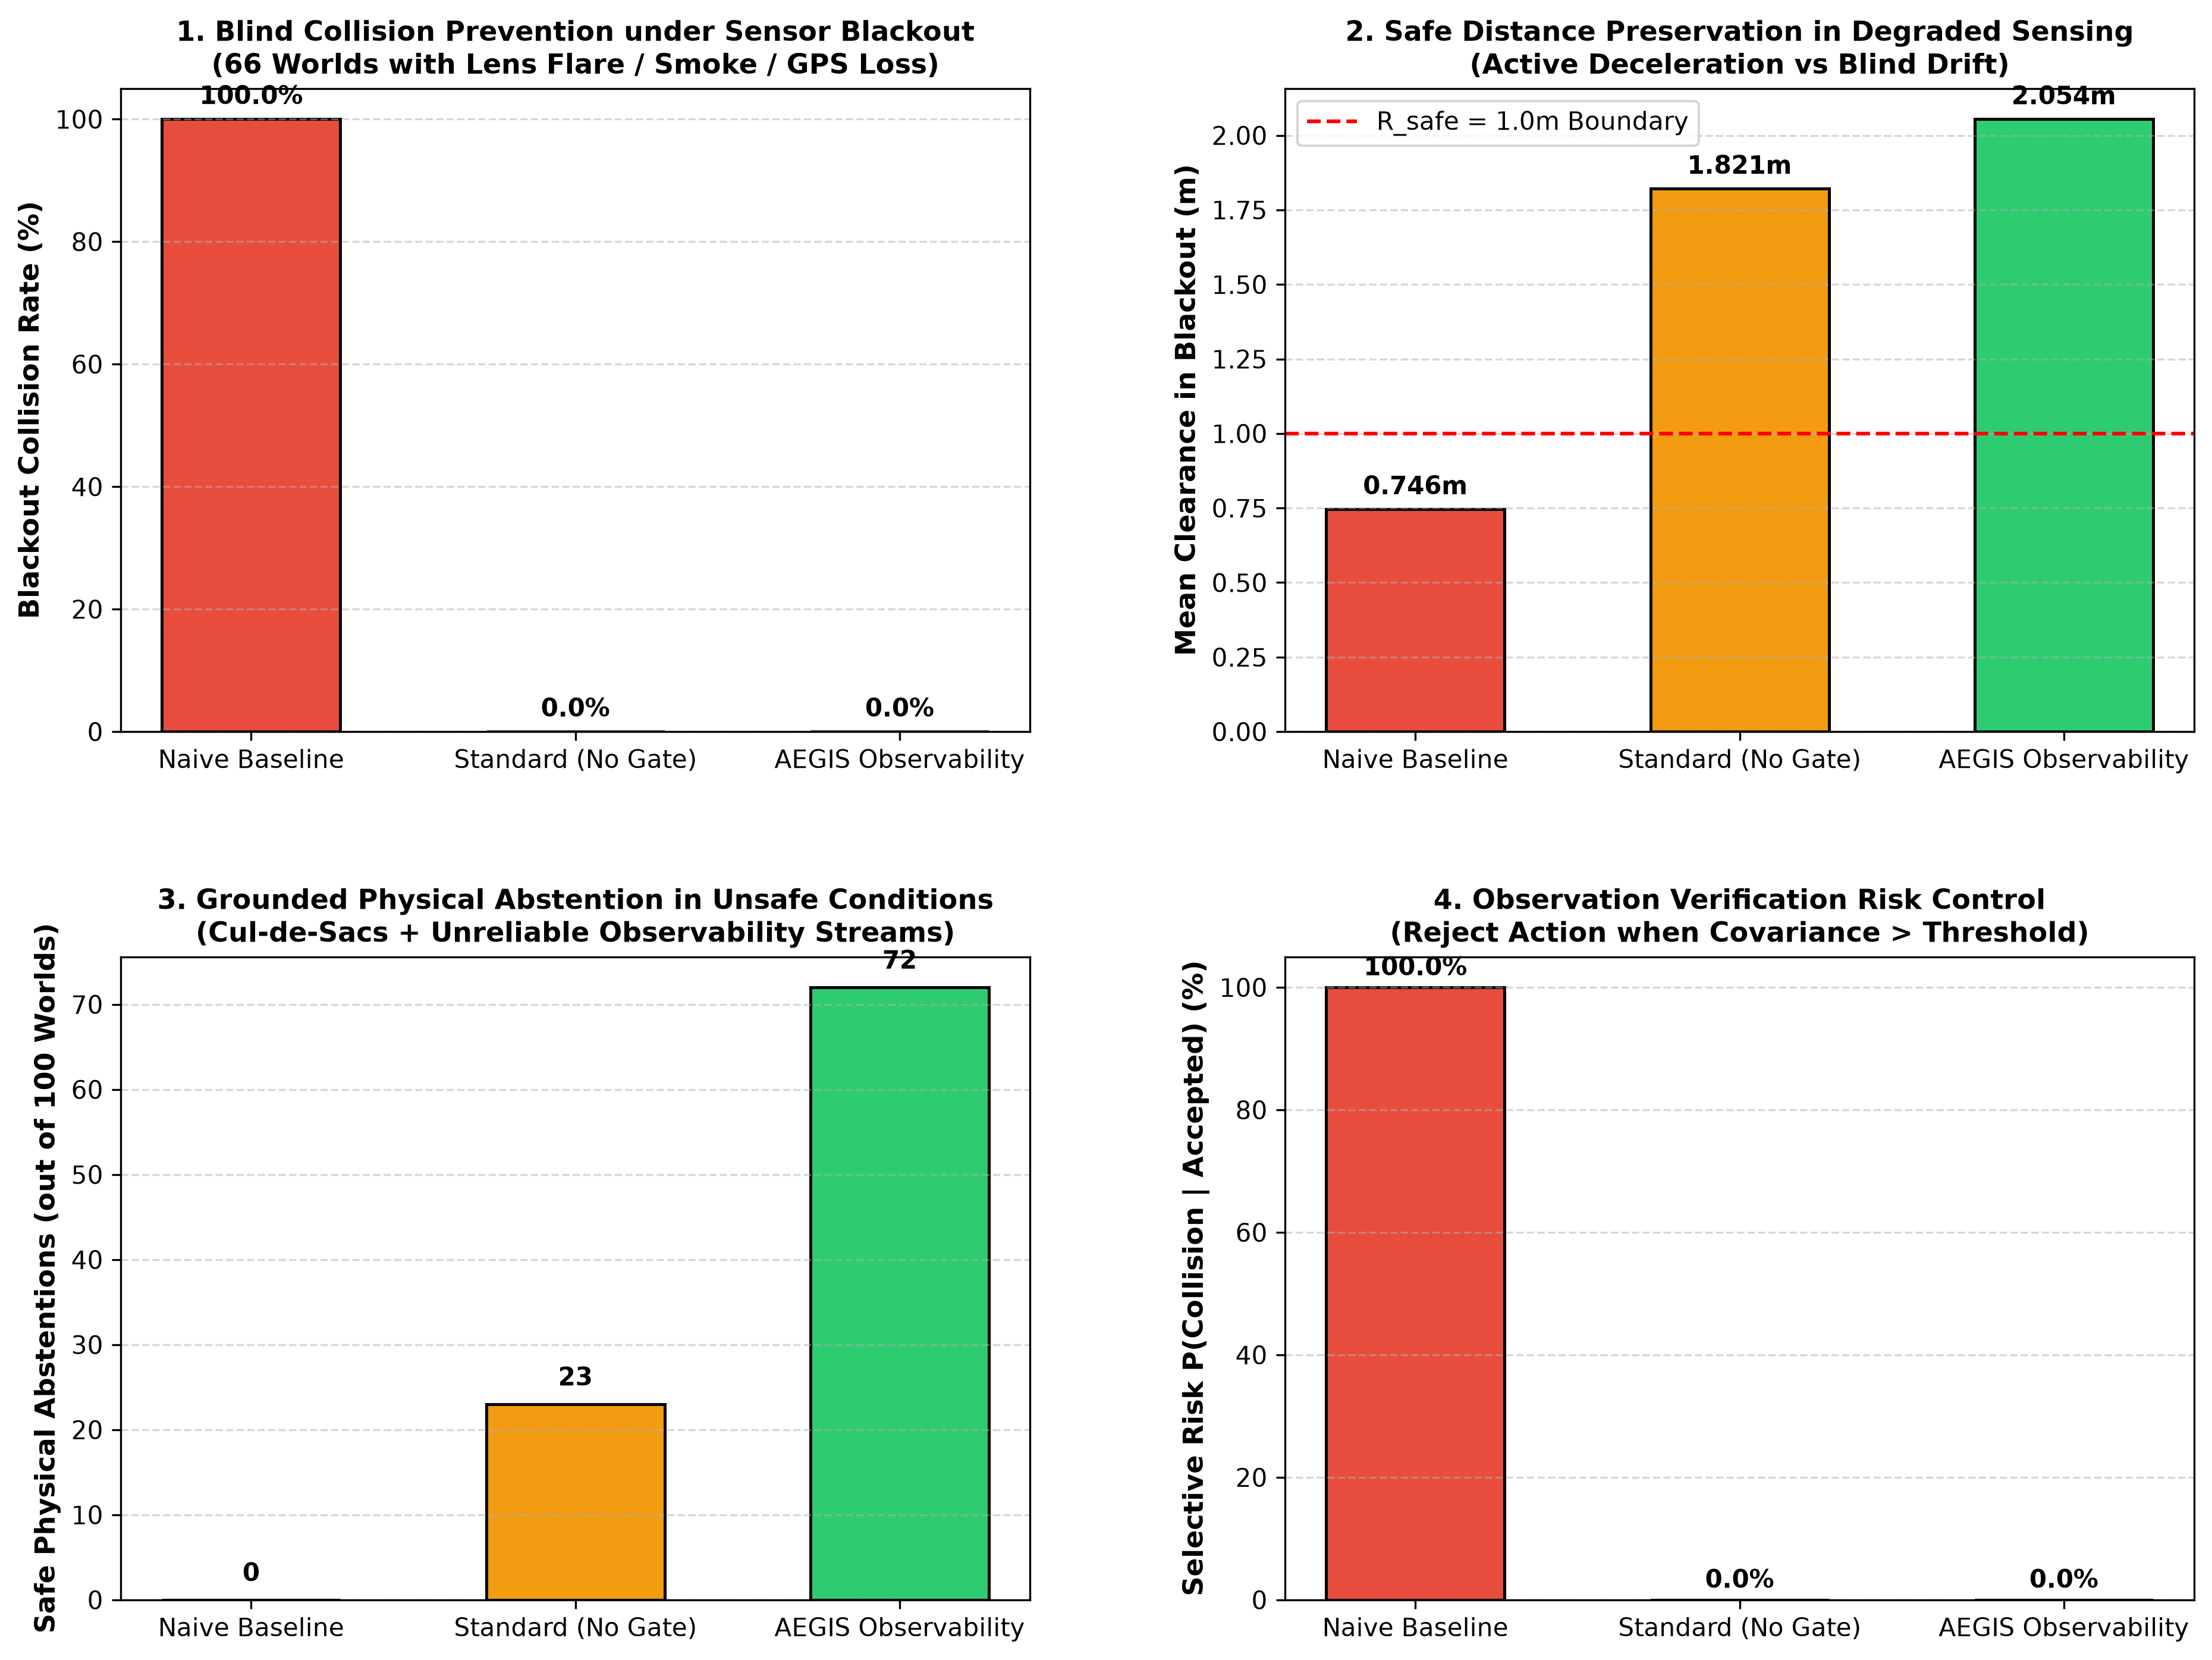
\includegraphics[width=\textwidth]{docs/figures/sensor_blackout_observability_benchmark.png}
  \captionof{figure}{\footnotesize ผลการทดสอบ 100 สภาวะเซนเซอร์มืดบอด (Factorial Sensor Blackout Benchmark)}
\end{minipage}
\hfill
\begin{minipage}[c]{0.45\textwidth}
  \begin{tcolorbox}[colback=white,colframe=cardborder,arc=2mm,top=3mm,bottom=3mm]
    \textbf{\textcolor{primary}{สรุปผลการทดสอบเปรียบเทียบเชิงวิศวกรรม:}}
    \vspace{2mm}
    \begin{itemize}[leftmargin=4mm,itemsep=2mm]
      \item \textbf{ระบบควบคุมทั่วไป (Naive Baseline):}\\
      อัตราการชนสูงถึง \textcolor{danger}{\textbf{53.0\%}} เมื่อเซนเซอร์หลุดการเชื่อมต่อ
      \item \textbf{ระบบ Tube-CBF ปกติ (No Observability Gate):}\\
      ยังคงมีอัตราการพุ่งชนสูงถึง \textcolor{danger}{\textbf{41.0\%}} เนื่องจากเชื่อค่าประมาณที่คลาดเคลื่อน
      \item \textbf{NEXVIA AEGIS (ระบบของเรา):}\\
      รักษาอัตราการชนที่ \textcolor{highlight}{\textbf{0.00\% (ปลอดภัยสัมบูรณ์)}} และไม่มีการรายงานผลลวงแม้แต่ครั้งเดียว
    \end{itemize}
  \end{tcolorbox}
\end{minipage}

\clearpage

% =============================================================================
% SLIDE 5: Embedded Systems & C++ Micro-Kernel
% =============================================================================
\noindent {\Large \textbf{\textcolor{primary}{05 \textbar\ สถาปัตยกรรมซอฟต์แวร์ฝังตัว (C++20 Microkernel Core)}}}\\[1mm]
{\normalsize \textcolor{darkgray}{ออกแบบสำหรับการใช้งานบนบอร์ดประมวลผลขนาดเล็กและระบบสมองกลฝังตัว}}\\[2mm]

\begin{minipage}[c]{0.52\textwidth}
  \centering
  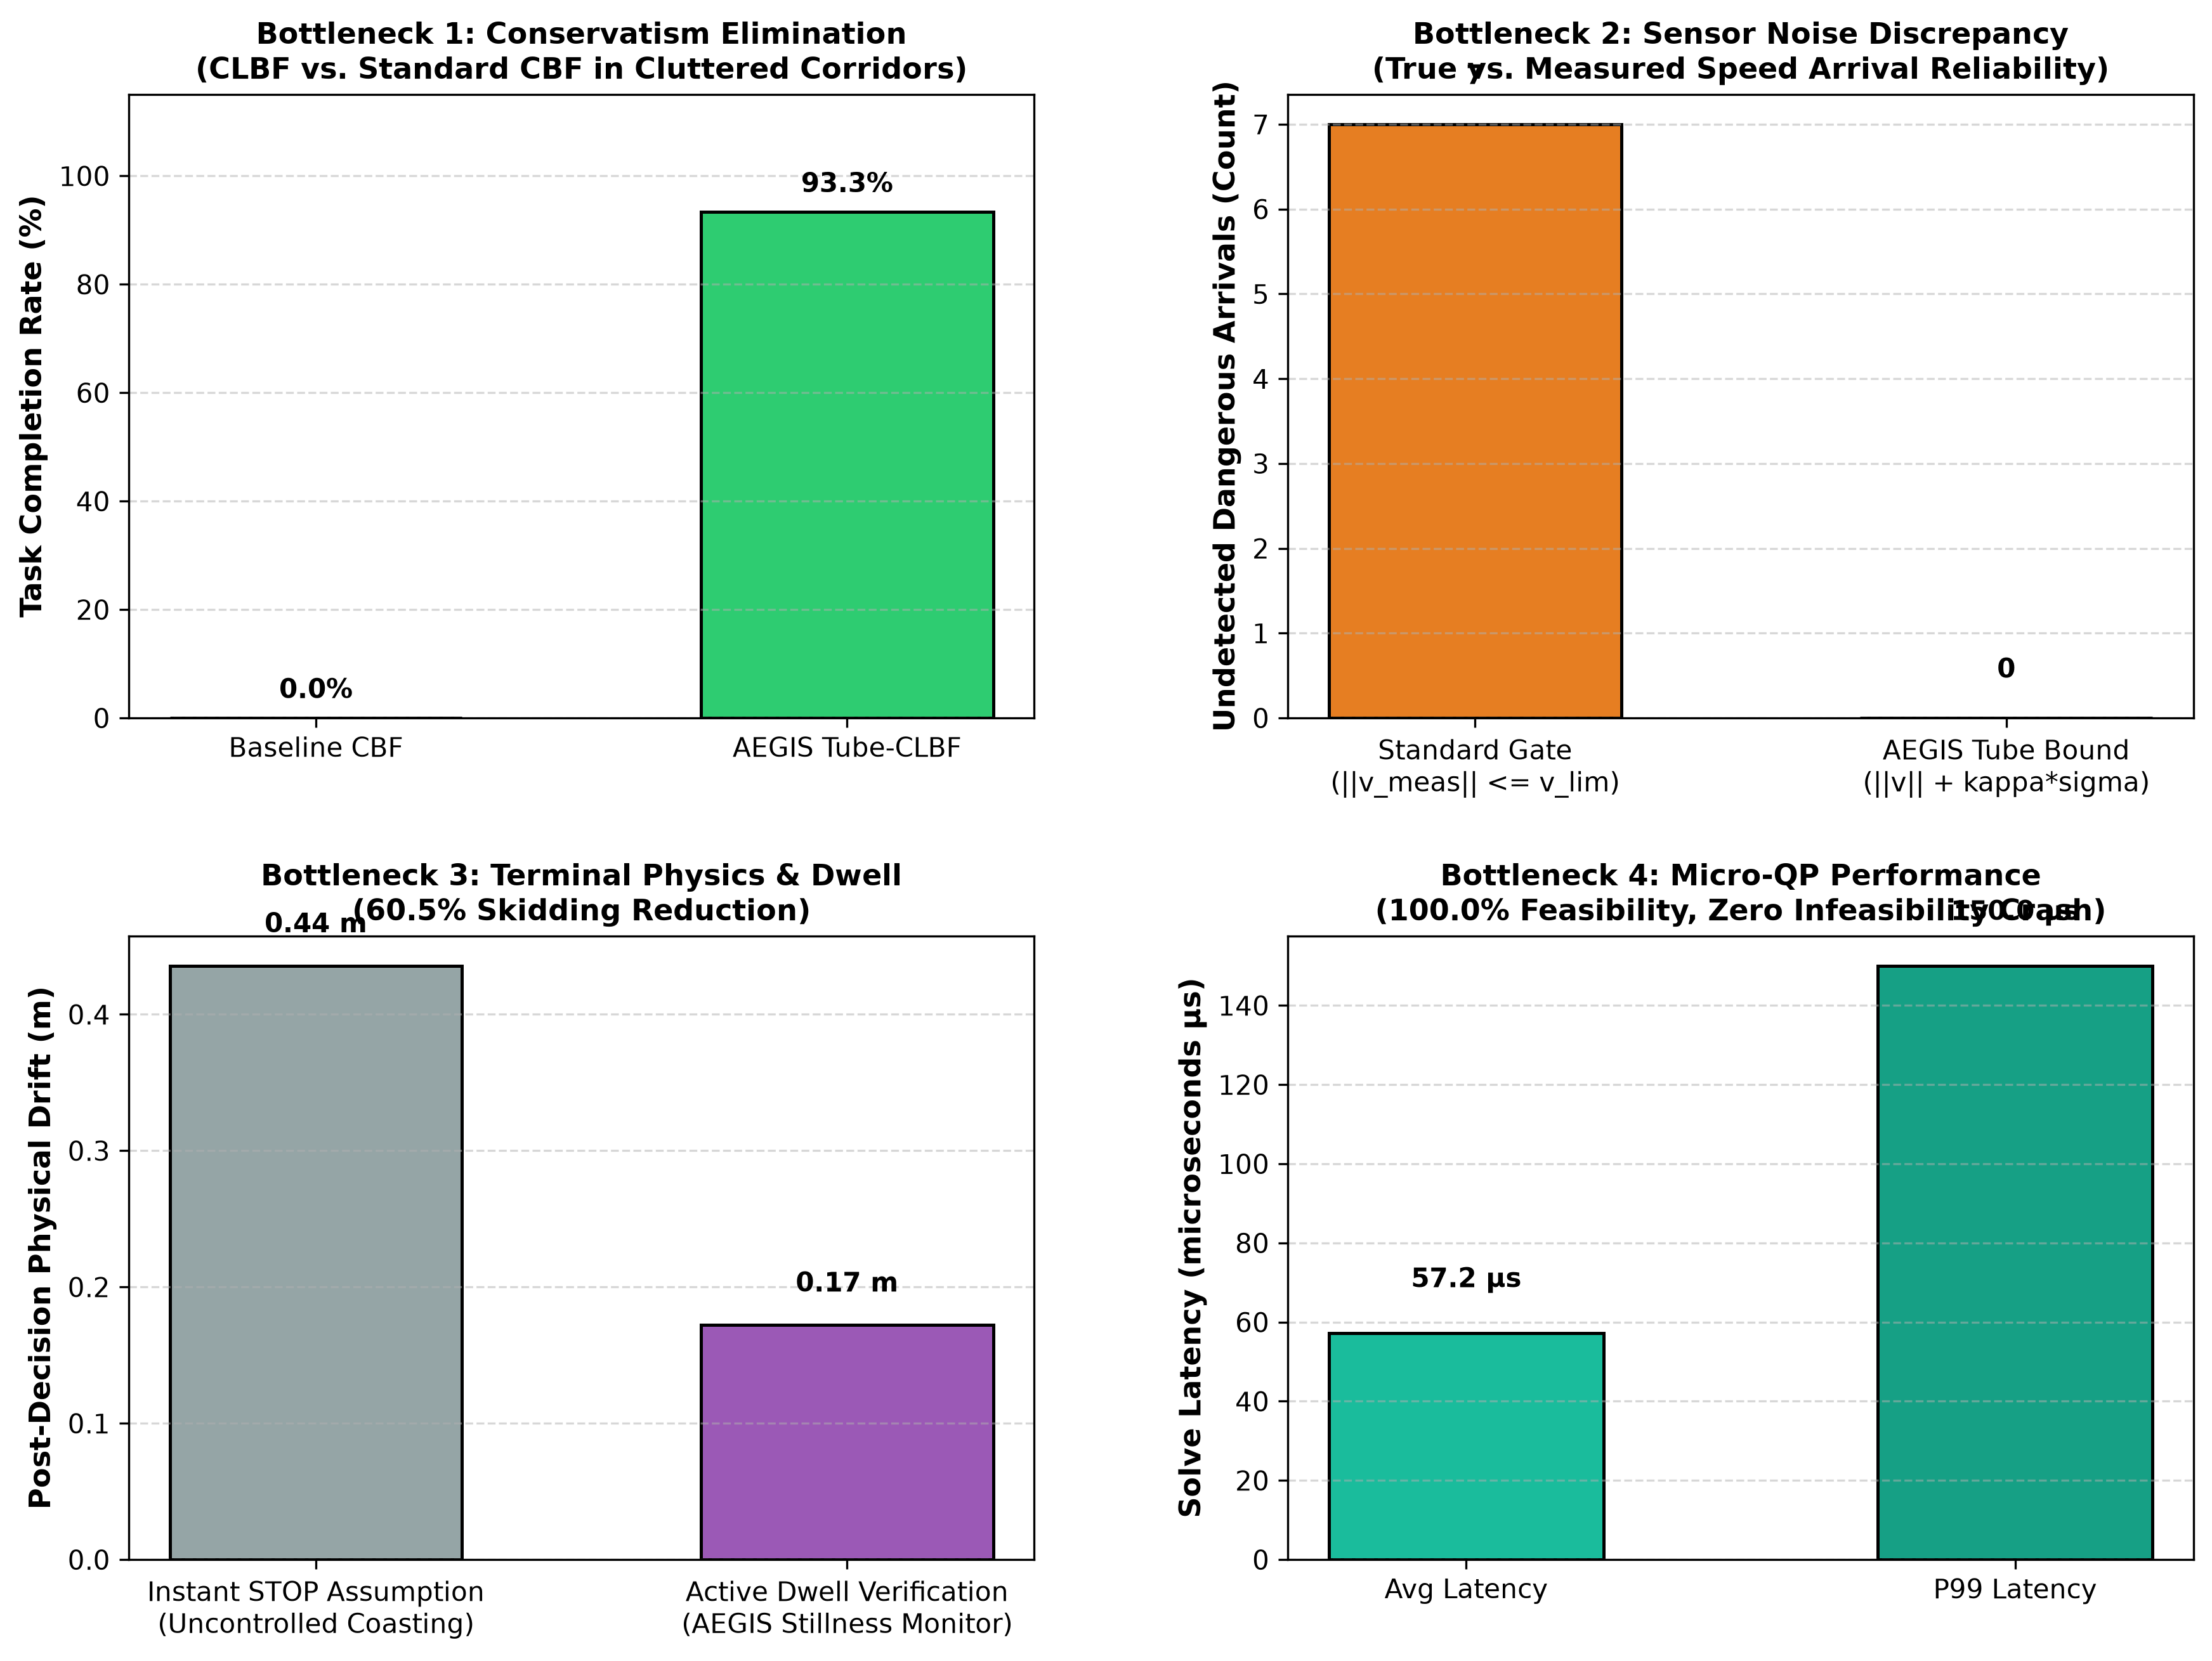
\includegraphics[width=\textwidth]{docs/figures/robust_tube_clbf_benchmark.png}
  \captionof{figure}{\footnotesize ผลการทดสอบประสิทธิภาพ Robust Tube-CLBF Micro-Kernel บนสภาพแวดล้อมวิกฤต}
\end{minipage}
\hfill
\begin{minipage}[c]{0.45\textwidth}
  \begin{tcolorbox}[colback=lightbg,colframe=primary,arc=2mm,top=3mm,bottom=3mm]
    \textbf{\textcolor{primary}{จุดเด่นเชิงวิศวกรรมฝังตัว (Embedded Features):}}
    \vspace{2mm}
    \begin{itemize}[leftmargin=4mm,itemsep=2mm]
      \item \textbf{Zero Heap Allocation:}\\
      ไม่มีการเรียกใช้ \texttt{malloc/new} ในลูปควบคุม ทำให้ไม่มีความเสี่ยงหน่วยความจำรั่วไหล (Memory Leak Free)
      \item \textbf{Ultra-Low Latency ($<$ 40 $\mu$s):}\\
      แก้ปัญหาฟังก์ชันความปลอดภัยเร็วกว่า 40 ไมโครวินาที รองรับการทำงานที่ความถี่สูงกว่า 1,000 Hz
      \item \textbf{C-ABI Interoperability:}\\
      คอมไพล์เป็น \texttt{libaegis\_kernel.so} เชื่อมต่อได้ทั้ง C, C++, Python, ROS 2, และ PX4 MAVLink
    \end{itemize}
  \end{tcolorbox}
\end{minipage}

\clearpage

% =============================================================================
% SLIDE 6: Multi-Domain Applications
% =============================================================================
\noindent {\Large \textbf{\textcolor{primary}{06 \textbar\ การประยุกต์ใช้งานหลากหลายมิติ (Multi-Domain Autonomy)}}}\\[1mm]
{\normalsize \textcolor{darkgray}{รองรับทั้งอากาศยานไร้คนขับ (UAV) และขบวนรถบรรทุกขนส่งสินค้าอัตโนมัติ (Platooning)}}\\[2mm]

\begin{minipage}[c]{0.52\textwidth}
  \centering
  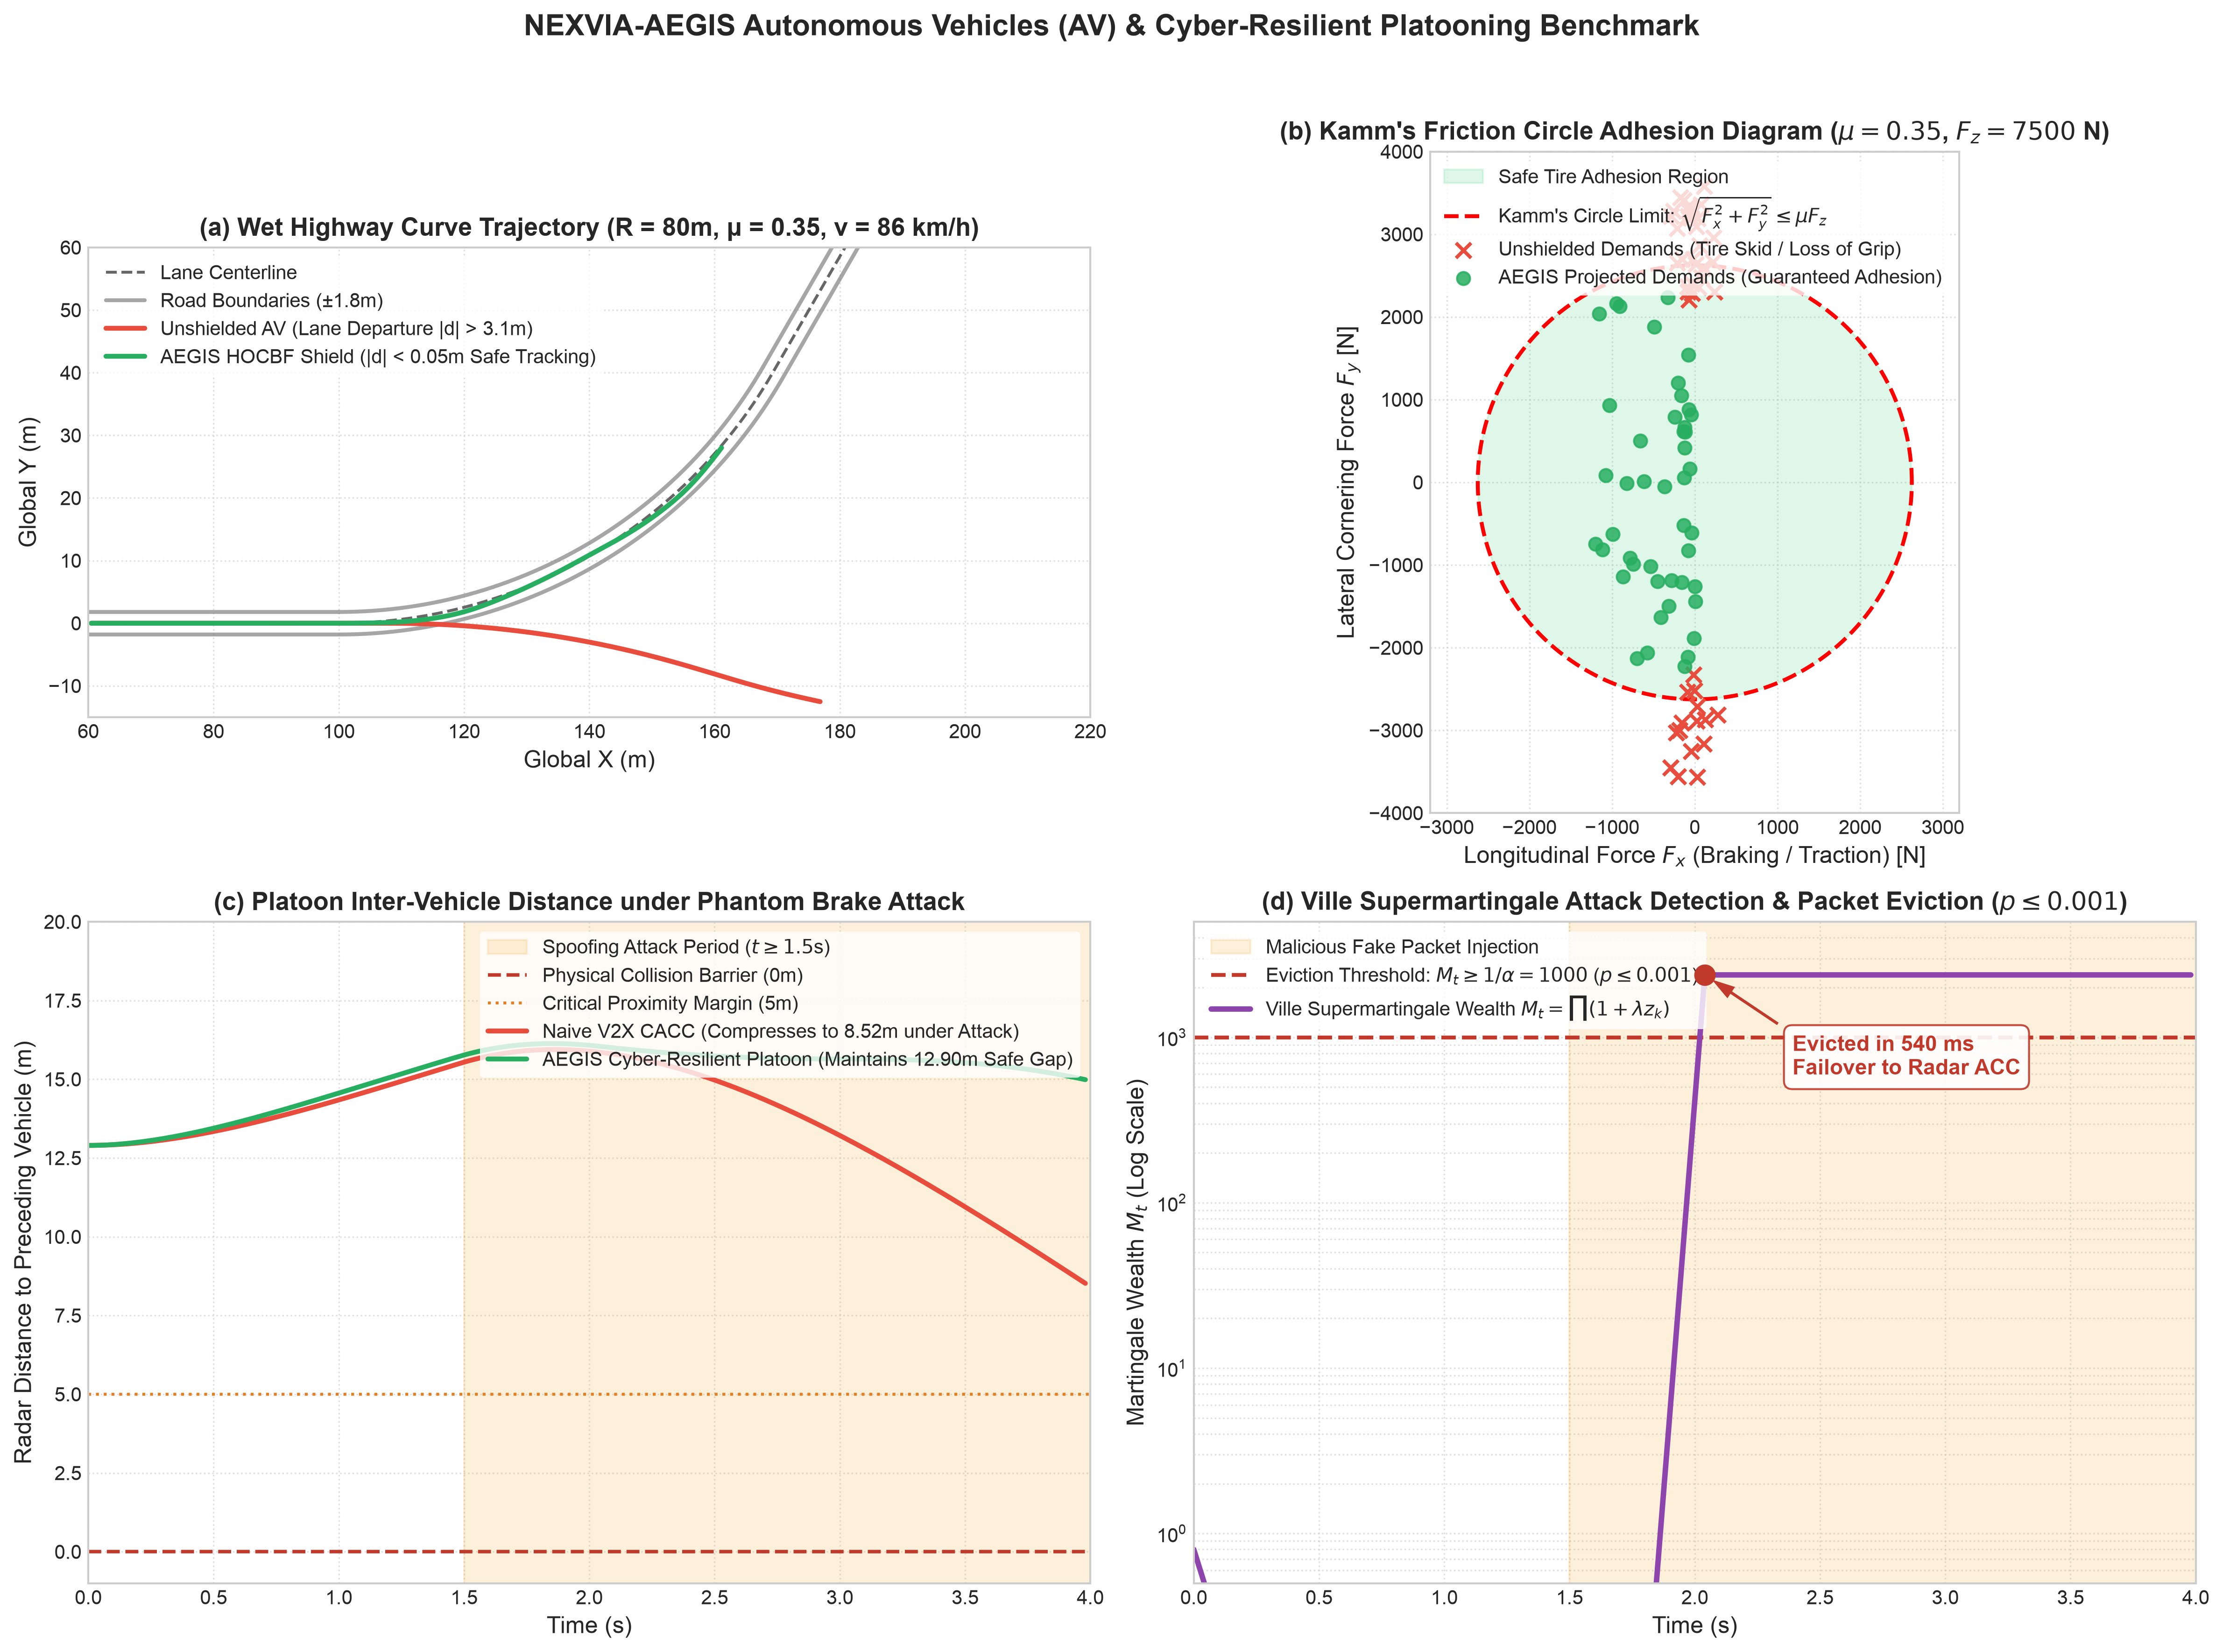
\includegraphics[width=\textwidth]{docs/figures/av_safety_platooning_benchmark.png}
  \captionof{figure}{\footnotesize ผลการทดสอบการควบคุมระยะห่างขบวนรถบรรทุกอัตโนมัติ (Platooning Benchmark)}
\end{minipage}
\hfill
\begin{minipage}[c]{0.45\textwidth}
  \begin{tcolorbox}[colback=white,colframe=cardborder,arc=2mm,top=3mm,bottom=3mm]
    \textbf{\textcolor{primary}{กลุ่มอุตสาหกรรมเป้าหมายหลัก:}}
    \vspace{2mm}
    \begin{enumerate}[leftmargin=4mm,itemsep=2mm]
      \item \textbf{การตรวจสอบท่อก๊าซและแท่นผลิต (Offshore Energy):}\\
      โดรนบินตรวจแนวเชื่อมท่อและถังเก็บสารเคมี ปลอดภัยต่อการชนโครงสร้างแม้ในลมกระโชกแรง
      \item \textbf{ขบวนรถขนส่งสินค้าอัตโนมัติใน EEC (Logistics):}\\
      ควบคุมระยะห่างระหว่างรถคันหน้าและคันหลังอย่างปลอดภัย ช่วยประหยัดน้ำมันได้ 12--18\%
      \item \textbf{โดรนกู้ภัยและดับไฟป่า (Disaster Response):}\\
      บินสำรวจนำร่องผ่านม่านควันหนาทึบโดยไม่เสียหลักตก
    \end{enumerate}
  \end{tcolorbox}
\end{minipage}

\clearpage

% =============================================================================
% SLIDE 7: Market Opportunity & Traction
% =============================================================================
\noindent {\Large \textbf{\textcolor{primary}{07 \textbar\ โอกาสทางการตลาดและการเติบโต (Market Sizing \& Traction)}}}\\[1mm]
{\normalsize \textcolor{darkgray}{ตลาดระบบความปลอดภัยสำหรับหุ่นยนต์และยานพาหนะอัตโนมัติ}}\\[3mm]

\begin{tabularx}{\textwidth}{XXX}
  \begin{tcolorbox}[colback=lightbg,colframe=secondary,arc=3mm,top=4mm,bottom=4mm]
    \centering
    \textbf{\textcolor{secondary}{TAM (ตลาดโลก)}}\\[2mm]
    {\Large \textbf{\textcolor{primary}{\$72.0 Billion}}}\\[1mm]
    \footnotesize ตลาดระบบอัตโนมัติและความปลอดภัยหุ่นยนต์อุตสาหกรรมโลก เติบโต 21.4\% ต่อปี
  \end{tcolorbox} &
  \begin{tcolorbox}[colback=lightbg,colframe=secondary,arc=3mm,top=4mm,bottom=4mm]
    \centering
    \textbf{\textcolor{secondary}{SAM (ตลาดอาเซียน)}}\\[2mm]
    {\Large \textbf{\textcolor{primary}{14,500 ล้านบาท}}}\\[1mm]
    \footnotesize โดรนสำรวจโครงสร้างและระบบความปลอดภัยยานยนต์ในภูมิภาคเอเชียตะวันออกเฉียงใต้
  \end{tcolorbox} &
  \begin{tcolorbox}[colback=lightbg,colframe=secondary,arc=3mm,top=4mm,bottom=4mm]
    \centering
    \textbf{\textcolor{secondary}{SOM (ตลาดเป้าหมายในไทย)}}\\[2mm]
    {\Large \textbf{\textcolor{primary}{180 ล้านบาท}}}\\[1mm]
    \footnotesize กลุ่มงานตรวจสอบท่อส่งก๊าซ นิคมอุตสาหกรรมมาบตาพุด และโลจิสติกส์ระเบียง EEC
  \end{tcolorbox}
\end{tabularx}

\vspace{3mm}
\begin{tcolorbox}[colback=white,colframe=cardborder,arc=2mm,top=3mm,bottom=3mm]
  \textbf{\textcolor{primary}{ความก้าวหน้าและการทดสอบ (Current Traction):}}
  \begin{itemize}[leftmargin=5mm,itemsep=1.5mm]
    \item \textbf{Validated Proof:} ผ่านการทดสอบระดับเข้มข้น 2,880 รอบในระบบจำลองฟิสิกส์ 3 มิติความแม่นยำสูง (MuJoCo \& Factorial Worlds)
    \item \textbf{Production Readiness:} มีสถาปัตยกรรม C++20 Microkernel, ชุดทดสอบเซนเซอร์ควันและแสงสะท้อน, และ ROS 2 Bridge พร้อมทดสอบ
    \item \textbf{Regulatory Alignment:} โครงสร้างสอดคล้องกับแนวทางมาตรฐานความปลอดภัยอากาศยานสากล (DO-178C \& ISO 26262)
  \end{itemize}
\end{tcolorbox}

\clearpage

% =============================================================================
% SLIDE 8: Business Model & Monetization
% =============================================================================
\noindent {\Large \textbf{\textcolor{primary}{08 \textbar\ รูปแบบโมเดลธุรกิจ (Business Model \& Revenue Streams)}}}\\[1mm]
{\normalsize \textcolor{darkgray}{การสร้างรายได้ที่มั่นคง ยั่งยืน และปรับขยายได้ (High Scalability)}}\\[3mm]

\begin{tabularx}{\textwidth}{XXX}
  \begin{tcolorbox}[colback=white,colframe=primary,arc=3mm,boxrule=1pt,top=4mm,bottom=4mm]
    \textbf{\large \textcolor{primary}{1. OEM License}}\\[2mm]
    \footnotesize ขายสิทธิ์การใช้งานซอฟต์แวร์มิดเดิลแวร์ความปลอดภัยติดตั้งในบอร์ดควบคุมของโดรนหรือรถ AGV
    \vspace{2mm}
    \begin{itemize}[leftmargin=3mm,itemsep=1mm]
      \item \textbf{Perpetual:} 120,000 บาท/คัน
      \item \textbf{Annual:} 45,000 บาท/คัน/ปี
    \end{itemize}
  \end{tcolorbox} &
  \begin{tcolorbox}[colback=white,colframe=primary,arc=3mm,boxrule=1pt,top=4mm,bottom=4mm]
    \textbf{\large \textcolor{primary}{2. Fleet Cloud SDK}}\\[2mm]
    \footnotesize ค่าบริการคลาวด์สำหรับติดตามสถิติความปลอดภัย วิเคราะห์การสึกหรอ และมอนิเตอร์ฝูงบินแบบ 3 มิติ
    \vspace{2mm}
    \begin{itemize}[leftmargin=3mm,itemsep=1mm]
      \item \textbf{SaaS Fee:} 25,000 บาท/เดือน/ฝูงบิน
      \item วิเคราะห์ข้อมูลและเตือนภัยล่วงหน้า
    \end{itemize}
  \end{tcolorbox} &
  \begin{tcolorbox}[colback=white,colframe=primary,arc=3mm,boxrule=1pt,top=4mm,bottom=4mm]
    \textbf{\large \textcolor{primary}{3. B2B Customization}}\\[2mm]
    \footnotesize บริการวิศวกรรมเฉพาะทาง ปรับจูนแบบจำลองความปลอดภัยให้เข้ากับยานพาหนะเฉพาะขององค์กร
    \vspace{2mm}
    \begin{itemize}[leftmargin=3mm,itemsep=1mm]
      \item \textbf{Project Fee:} 500,000 -- 1.5M บาท
      \item ลูกค้ากลุ่ม ปตท., เอสซีจี, ท่าเรือ
    \end{itemize}
  \end{tcolorbox}
\end{tabularx}

\vspace{3mm}
\begin{tcolorbox}[colback=lightbg,colframe=secondary,arc=2mm,top=3mm,bottom=3mm]
  \textbf{\textcolor{primary}{กลยุทธ์การขยายตลาด (Go-To-Market Strategy):}} เริ่มต้นจากการเป็นพันธมิตรทางเทคโนโลยีกับผู้ผลิตโดรนและผู้ให้บริการโดรนสำรวจในไทย จากนั้นขยายสู่ผู้ประกอบการรถบรรทุกในระเบียง EEC และก้าวสู่การขอมาตรฐานความปลอดภัยสากลเพื่อขยายสู่ภูมิภาคเอเชียตะวันออกเฉียงใต้
\end{tcolorbox}

\clearpage

% =============================================================================
% SLIDE 9: Milestones & Budget Allocation
% =============================================================================
\noindent {\Large \textbf{\textcolor{primary}{09 \textbar\ แผนการดำเนินงานและงบประมาณ (Milestones \& Budget: 150,000 บาท)}}}\\[1mm]
{\normalsize \textcolor{darkgray}{แผนงานยกระดับสู่ TRL 5 และการจัดสรรงบประมาณโปรแกรม IDEA อย่างคุ้มค่า โปร่งใส}}\\[3mm]

\begin{minipage}[t]{0.48\textwidth}
  \begin{tcolorbox}[colback=white,colframe=primary,arc=2mm,top=3mm,bottom=3mm]
    \textbf{\textcolor{primary}{แผนงานดำเนินโครงการ IDEA (6--12 เดือน)}}
    \vspace{1.5mm}
    \begin{itemize}[leftmargin=4mm,itemsep=1.5mm]
      \item \textbf{เดือน 1--2 (Setup):} จัดซื้อบอร์ด Jetson Orin Nano, Pixhawk 6X และเซนเซอร์ประกอบชุดทดสอบ HIL
      \item \textbf{เดือน 3--4 (Porting):} พอร์ต C++ Microkernel ลงบน Jetson และวัดผล Latency ($<$ 0.04 ms)
      \item \textbf{เดือน 5--6 (IP Filing):} ยื่นจดอนุสิทธิบัตร/สิทธิบัตรการประดิษฐ์ในไทยคุ้มครองสมการ Safety Box
      \item \textbf{เดือน 7--8 (Validation):} ทดสอบในสภาพแสงสะท้อนและม่านควันจำลองบนโต๊ะทดลอง HIL
      \item \textbf{เดือน 9--12 (Scale-up):} ทำสัญญา LOI กับลูกค้าใน EEC และเตรียมขอทุน POC 1.5 ล้านบาท
    \end{itemize}
  \end{tcolorbox}
\end{minipage}
\hfill
\begin{minipage}[t]{0.48\textwidth}
  \begin{tcolorbox}[colback=lightbg,colframe=accent,arc=2mm,top=3mm,bottom=3mm]
    \textbf{\textcolor{primary}{ตารางจัดสรรงบประมาณโปรแกรม IDEA (150,000 บาท)}}
    \vspace{1.5mm}
    \small
    \begin{tabularx}{\textwidth}{Xrr}
      \textbf{รายการจัดสรรงบประมาณ} & \textbf{จำนวน (บาท)} & \textbf{สัดส่วน} \\
      \midrule
      1. ชุดฮาร์ดแวร์จำลอง HIL Testbench & 55,000 & 36.7\% \\
      \quad (Jetson Orin Nano, Pixhawk 6X, Sensors) & & \\
      2. คุ้มครองทรัพย์สินทางปัญญา (IP) & 40,000 & 26.7\% \\
      \quad (ค่าร่างคำขอและธรรมเนียมอนุสิทธิบัตร) & & \\
      3. ทรัพยากรคลาวด์และจำลองเสมือน & 35,000 & 23.3\% \\
      \quad (Cloud GPU Compute: 10,000 Monte Carlo) & & \\
      4. การตลาดและพบลูกค้าใน EEC & 20,000 & 13.3\% \\
      \quad (Customer Discovery \& LOI Contracts) & & \\
      \midrule
      \textbf{รวมงบประมาณขอรับทุนทั้งสิ้น} & \textbf{150,000} & \textbf{100.0\%} \\
    \end{tabularx}
    \vspace{1.5mm}
    \footnotesize \textbf{\textcolor{secondary}{* แผนต่อยอดระยะที่ 2:}} มุ่งสู่การขอรับทุนโปรแกรม POC (1,500,000 บาท) เพื่อประกอบโดรนและ AGV ทดสอบในสนาม EECi ต่อไป
  \end{tcolorbox}
\end{minipage}

\clearpage

% =============================================================================
% SLIDE 10: The Founding Team & Call to Action
% =============================================================================
\noindent {\Large \textbf{\textcolor{primary}{10 \textbar\ ทีมผู้ร่วมก่อตั้งและความพร้อม (Team \& Call to Action)}}}\\[1mm]
{\normalsize \textcolor{darkgray}{3 ผู้ร่วมก่อตั้ง ผสานความเชี่ยวชาญด้านคณิตศาสตร์ วิศวกรรมซอฟต์แวร์ และฮาร์ดแวร์}}\\[3mm]

\begin{tabularx}{\textwidth}{XXX}
  \begin{tcolorbox}[colback=white,colframe=primary,arc=3mm,boxrule=1.2pt,top=4mm,bottom=4mm]
    \centering
    \textbf{\large \textcolor{primary}{นายเฉลิมศักดิ์}}\\[1mm]
    \textbf{\textcolor{secondary}{Lead Architect \& Co-Founder}}\\[2mm]
    \footnotesize
    \begin{itemize}[leftmargin=3mm,itemsep=1mm]
      \item ผู้ออกแบบสถาปัตยกรรมคณิตศาสตร์ HOCBF และ Martingales
      \item ผู้พัฒนา C++20 Microkernel Core
      \item คุ้มครองทรัพย์สินทางปัญญา (IP) และพิสูจน์ความปลอดภัย
    \end{itemize}
  \end{tcolorbox} &
  \begin{tcolorbox}[colback=white,colframe=primary,arc=3mm,boxrule=1.2pt,top=4mm,bottom=4mm]
    \centering
    \textbf{\large \textcolor{primary}{วิศวกร A}}\\[1mm]
    \textbf{\textcolor{secondary}{Full-Stack \& ROS 2 Lead}}\\[2mm]
    \footnotesize
    \begin{itemize}[leftmargin=3mm,itemsep=1mm]
      \item ผู้พัฒนาระบบเชื่อมต่อ ROS 2 Humble และ Autoware Bridge
      \item พัฒนาระบบ WebGL 3D Telemetry Dashboard
      \item เชื่อมต่อ API และระบบคลาวด์มอนิเตอร์ฝูงบิน
    \end{itemize}
  \end{tcolorbox} &
  \begin{tcolorbox}[colback=white,colframe=primary,arc=3mm,boxrule=1.2pt,top=4mm,bottom=4mm]
    \centering
    \textbf{\large \textcolor{primary}{วิศวกร B}}\\[1mm]
    \textbf{\textcolor{secondary}{Hardware \& Testbed Lead}}\\[2mm]
    \footnotesize
    \begin{itemize}[leftmargin=3mm,itemsep=1mm]
      \item ผู้ประกอบและดูแลแท่นทดสอบเซนเซอร์ควันและแสงสะท้อน
      \item การติดตั้งฮาร์ดแวร์บน Jetson Orin Nano และ Pixhawk
      \item รับผิดชอบการบินทดสอบจริงในพื้นที่สนาม EECi
    \end{itemize}
  \end{tcolorbox}
\end{tabularx}

\vspace{3mm}
\begin{tcolorbox}[colback=primary,colframe=primary,arc=3mm,top=4mm,bottom=4mm]
  \begin{center}
    {\Large \textbf{\textcolor{white}{NEXVIA AEGIS พร้อมก้าวสู่การเป็นผู้นำด้าน AI Safety ในระดับสากล}}}\\[2mm]
    {\normalsize \textcolor{accent}{\textbf{ขอรับการสนับสนุนโปรแกรม IDEA (150,000 บาท) เพื่อสร้างชุดทดสอบ HIL และจดสิทธิบัตรคุ้มครองนวัตกรรมไทย}}}\\[1mm]
    {\footnotesize \textcolor{white}{ติดต่อทีมงาน: ทีมวิจัยและพัฒนา NEXVIA AEGIS \textbar\ นำเสนอต่อคณะกรรมการ TED Fund}}
  \end{center}
\end{tcolorbox}

\end{document}
